\documentclass{article}
\usepackage{tikz}
\usetikzlibrary{patterns}
\usepackage{caption}
\usepackage{subcaption}
\usepackage{geometry}
\geometry{a4paper, margin=1in}
\begin{document}

\begin{figure}[htbp]
    \centering
    \begin{subfigure}[b]{0.27\textwidth}
        \centering
        \resizebox{\linewidth}{!}{        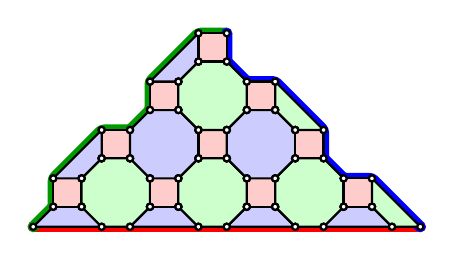
\begin{tikzpicture}[scale=0.45]
            \pgfdeclarelayer{background}
            \pgfsetlayers{background,main}
            \def\L{1.3657} 
            \colorlet{colR}{red!20} \colorlet{colG}{green!20} \colorlet{colB}{blue!20}
            
            \newcommand{\simplsq}[2]{
                \filldraw[fill=colR, draw=black, thick] ({#1-0.4},{#2-0.4}) rectangle ({#1+0.4},{#2+0.4});
            }
            \newcommand{\simploct}[3]{
                \filldraw[fill=#3, draw=black, thick]
                    ({#1-0.4},{#2-0.9657}) -- ({#1+0.4},{#2-0.9657}) -- ({#1+0.9657},{#2-0.4}) --
                    ({#1+0.9657},{#2+0.4}) -- ({#1+0.4},{#2+0.9657}) -- ({#1-0.4},{#2+0.9657}) --
                    ({#1-0.9657},{#2+0.4}) -- ({#1-0.9657},{#2-0.4}) -- cycle;
            }
            \newcommand{\simpltrapBtop}[2]{
                \filldraw[fill=colB, draw=black, thick]
                    ({#1-0.9657},{#2+0.4}) -- ({#1-0.4},{#2+0.9657}) -- 
                    ({#1+0.4},{#2+0.9657}) -- ({#1+0.9657},{#2+0.4}) -- cycle;
            }
            \newcommand{\simpltrapBright}[2]{
                \filldraw[fill=colB, draw=black, thick]
                    ({#1+0.9657},{#2+0.4}) -- ({#1+0.9657},{#2-0.4}) -- 
                    ({#1+0.4},{#2-0.9657}) -- ({#1-0.4},{#2-0.9657}) -- cycle;
            }
            \newcommand{\simpltrapGleft}[2]{
                \filldraw[fill=colG, draw=black, thick]
                    ({#1-0.9657},{#2+0.4}) -- ({#1-0.9657},{#2-0.4}) -- 
                    ({#1-0.4},{#2-0.9657}) -- ({#1+0.4},{#2-0.9657}) -- cycle;
            }
            
            \newcommand{\fullsqqubits}[2]{
                \filldraw[fill=white, draw=black, thick] ({#1-0.4},{#2-0.4}) circle (2.5pt);
                \filldraw[fill=white, draw=black, thick] ({#1+0.4},{#2-0.4}) circle (2.5pt);
                \filldraw[fill=white, draw=black, thick] ({#1+0.4},{#2+0.4}) circle (2.5pt);
                \filldraw[fill=white, draw=black, thick] ({#1-0.4},{#2+0.4}) circle (2.5pt);
            }
            \newcommand{\fulloctqubits}[2]{
                \filldraw[fill=white, draw=black, thick] ({#1-0.4},{#2-0.9657}) circle (2.5pt);
                \filldraw[fill=white, draw=black, thick] ({#1+0.4},{#2-0.9657}) circle (2.5pt);
                \filldraw[fill=white, draw=black, thick] ({#1+0.9657},{#2-0.4}) circle (2.5pt);
                \filldraw[fill=white, draw=black, thick] ({#1+0.9657},{#2+0.4}) circle (2.5pt);
                \filldraw[fill=white, draw=black, thick] ({#1+0.4},{#2+0.9657}) circle (2.5pt);
                \filldraw[fill=white, draw=black, thick] ({#1-0.4},{#2+0.9657}) circle (2.5pt);
                \filldraw[fill=white, draw=black, thick] ({#1-0.9657},{#2+0.4}) circle (2.5pt);
                \filldraw[fill=white, draw=black, thick] ({#1-0.9657},{#2-0.4}) circle (2.5pt);
            }
            \newcommand{\trapBtopqubits}[2]{
                \filldraw[fill=white, draw=black, thick] ({#1-0.9657},{#2+0.4}) circle (2.5pt);
                \filldraw[fill=white, draw=black, thick] ({#1-0.4},{#2+0.9657}) circle (2.5pt);
                \filldraw[fill=white, draw=black, thick] ({#1+0.4},{#2+0.9657}) circle (2.5pt);
                \filldraw[fill=white, draw=black, thick] ({#1+0.9657},{#2+0.4}) circle (2.5pt);
            }
            \newcommand{\trapBrightqubits}[2]{
                \filldraw[fill=white, draw=black, thick] ({#1+0.9657},{#2+0.4}) circle (2.5pt);
                \filldraw[fill=white, draw=black, thick] ({#1+0.9657},{#2-0.4}) circle (2.5pt);
                \filldraw[fill=white, draw=black, thick] ({#1+0.4},{#2-0.9657}) circle (2.5pt);
                \filldraw[fill=white, draw=black, thick] ({#1-0.4},{#2-0.9657}) circle (2.5pt);
            }
            \newcommand{\trapGleftqubits}[2]{
                \filldraw[fill=white, draw=black, thick] ({#1-0.9657},{#2+0.4}) circle (2.5pt);
                \filldraw[fill=white, draw=black, thick] ({#1-0.9657},{#2-0.4}) circle (2.5pt);
                \filldraw[fill=white, draw=black, thick] ({#1-0.4},{#2-0.9657}) circle (2.5pt);
                \filldraw[fill=white, draw=black, thick] ({#1+0.4},{#2-0.9657}) circle (2.5pt);
            }

            \simpltrapBtop{-3*\L}{0}
            \simpltrapBtop{-\L}{0}
            \simpltrapBtop{\L}{0}
            \simpltrapBtop{3*\L}{0}

            \simplsq{-3*\L}{\L}
            \simploct{-2*\L}{\L}{colG}
            \simplsq{-\L}{\L}
            \simploct{0}{\L}{colG}
            \simplsq{\L}{\L}
            \simploct{2*\L}{\L}{colG}
            \simplsq{3*\L}{\L}
            \simpltrapGleft{4*\L}{\L}

            \simpltrapBright{-3*\L}{2*\L}
            \simplsq{-2*\L}{2*\L}
            \simploct{-\L}{2*\L}{colB}
            \simplsq{0}{2*\L}
            \simploct{\L}{2*\L}{colB}
            \simplsq{2*\L}{2*\L}

            \simplsq{-\L}{3*\L}
            \simploct{0}{3*\L}{colG}
            \simplsq{\L}{3*\L}
            \simpltrapGleft{2*\L}{3*\L}

            \simpltrapBright{-\L}{4*\L}
            \simplsq{0}{4*\L}






            \trapBtopqubits{-3*\L}{0}
            \trapBtopqubits{-\L}{0}
            \trapBtopqubits{\L}{0}
            \trapBtopqubits{3*\L}{0}

            \fullsqqubits{-3*\L}{\L}
            \fulloctqubits{-2*\L}{\L}
            \fullsqqubits{-\L}{\L}
            \fulloctqubits{0}{\L}
            \fullsqqubits{\L}{\L}
            \fulloctqubits{2*\L}{\L}
            \fullsqqubits{3*\L}{\L}
            \trapGleftqubits{4*\L}{\L}

            \trapBrightqubits{-3*\L}{2*\L}
            \fullsqqubits{-2*\L}{2*\L}
            \fulloctqubits{-\L}{2*\L}
            \fullsqqubits{0}{2*\L}
            \fulloctqubits{\L}{2*\L}
            \fullsqqubits{2*\L}{2*\L}

            \fullsqqubits{-\L}{3*\L}
            \fulloctqubits{0}{3*\L}
            \fullsqqubits{\L}{3*\L}
            \trapGleftqubits{2*\L}{3*\L}

            \trapBrightqubits{-\L}{4*\L}
            \fullsqqubits{0}{4*\L}

            \begin{pgfonlayer}{background}
                \draw[red, line width=4pt, line cap=round] 
                    ({-3*\L-0.9657}, 0.4) -- ({4*\L+0.4}, 0.4);

                \draw[green!60!black, line width=4pt, rounded corners=1pt, line cap=round]
                    ({-3*\L-0.9657}, 0.4) 
                    -- ({-3*\L-0.4}, 0.9657)
                    -- ({-3*\L-0.4}, {\L+0.4})
                    -- ({-2*\L-0.4}, {2*\L+0.4})
                    -- ({-2*\L+0.4}, {2*\L+0.4})
                    -- ({-\L-0.4}, {3*\L-0.4})
                    -- ({-\L-0.4}, {3*\L+0.4})
                    -- ({-0.4}, {4*\L+0.4})
                    -- ({0.4}, {4*\L+0.4});

                \draw[blue, line width=4pt, rounded corners=1pt, line cap=round]
                    ({4*\L+0.4}, 0.4)
                    -- ({3*\L+0.4}, {\L+0.4})
                    -- ({3*\L-0.4}, {\L+0.4})
                    -- ({2*\L+0.4}, {2*\L-0.4})
                    -- ({2*\L+0.4}, {2*\L+0.4})
                    -- ({\L+0.4}, {3*\L+0.4})
                    -- ({\L-0.4}, {3*\L+0.4})
                    -- ({0.4}, {4*\L-0.4})
                    -- ({0.4}, {4*\L+0.4});
            \end{pgfonlayer}

        \end{tikzpicture}
}
        \caption{Original color code lattice}
        \label{fig:mobius_a}
    \end{subfigure}
    \hfill
    \begin{subfigure}[b]{0.27\textwidth}
        \centering
        \resizebox{\linewidth}{!}{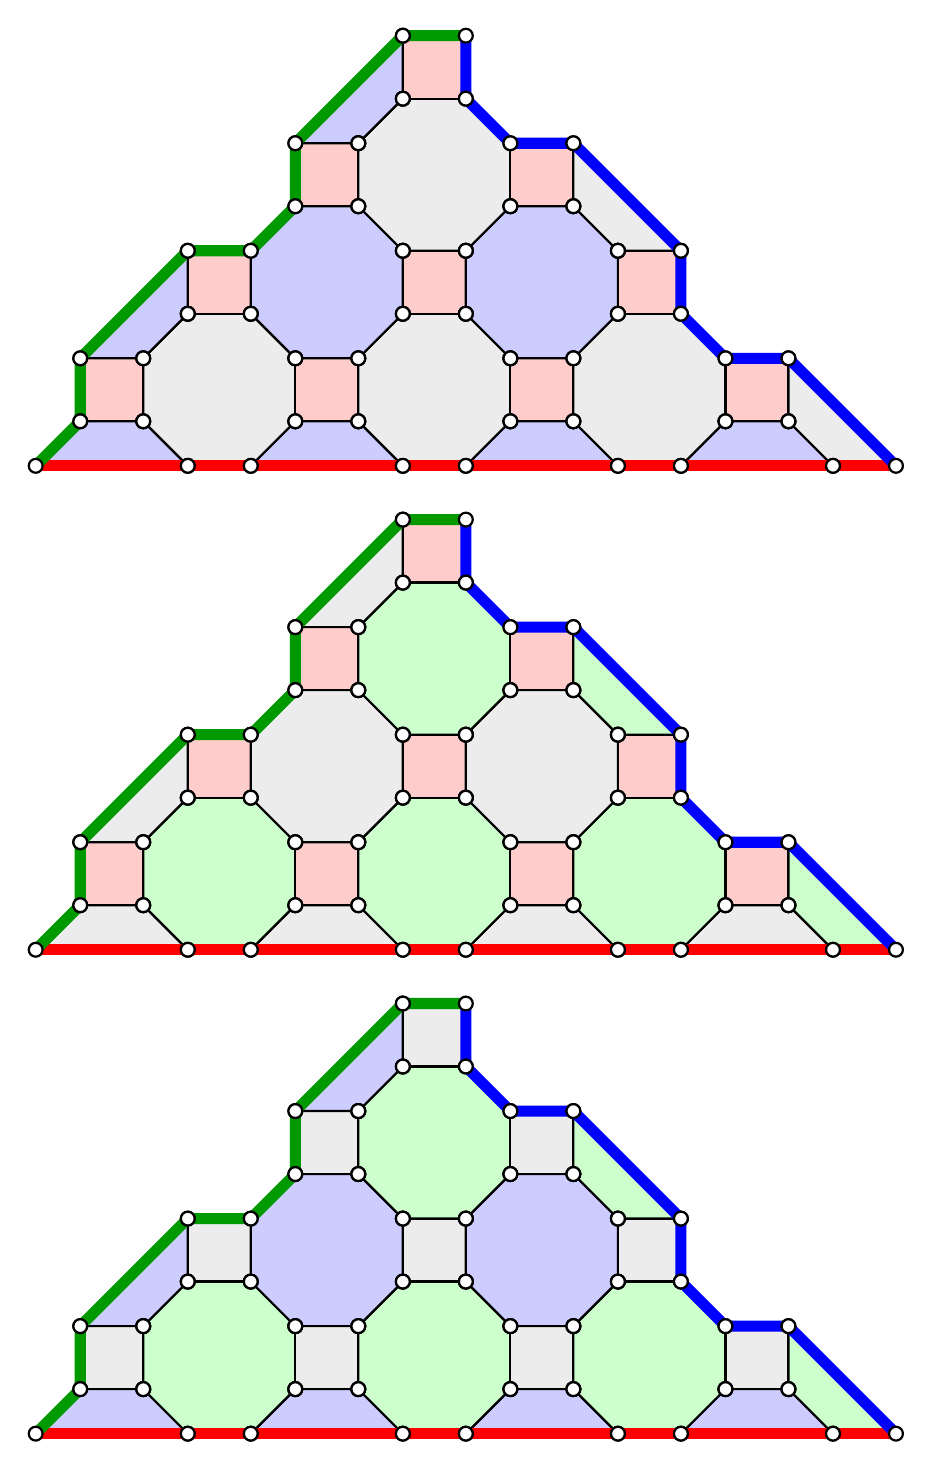
\begin{tikzpicture}
\def\L{1.3657}

\newcommand{\simplsq}[2]{
                \filldraw[colR] ({#1-0.4},{#2-0.4}) rectangle ({#1+0.4},{#2+0.4});
            }
            \newcommand{\simploct}[3]{
                \filldraw[#3]
                    ({#1-0.4},{#2-0.9657}) -- ({#1+0.4},{#2-0.9657}) -- ({#1+0.9657},{#2-0.4}) --
                    ({#1+0.9657},{#2+0.4}) -- ({#1+0.4},{#2+0.9657}) -- ({#1-0.4},{#2+0.9657}) --
                    ({#1-0.9657},{#2+0.4}) -- ({#1-0.9657},{#2-0.4}) -- cycle;
            }
            \newcommand{\simpltrapBtop}[2]{
                \filldraw[colB]
                    ({#1-0.9657},{#2+0.4}) -- ({#1-0.4},{#2+0.9657}) -- 
                    ({#1+0.4},{#2+0.9657}) -- ({#1+0.9657},{#2+0.4}) -- cycle;
            }
            \newcommand{\simpltrapBright}[2]{
                \filldraw[colB]
                    ({#1+0.9657},{#2+0.4}) -- ({#1+0.9657},{#2-0.4}) -- 
                    ({#1+0.4},{#2-0.9657}) -- ({#1-0.4},{#2-0.9657}) -- cycle;
            }
            \newcommand{\simpltrapGleft}[2]{
                \filldraw[colG]
                    ({#1-0.9657},{#2+0.4}) -- ({#1-0.9657},{#2-0.4}) -- 
                    ({#1-0.4},{#2-0.9657}) -- ({#1+0.4},{#2-0.9657}) -- cycle;
            }
            
            \newcommand{\fullsqqubits}[2]{
                \filldraw[fill=white, draw=black, thick] ({#1-0.4},{#2-0.4}) circle (2.5pt);
                \filldraw[fill=white, draw=black, thick] ({#1+0.4},{#2-0.4}) circle (2.5pt);
                \filldraw[fill=white, draw=black, thick] ({#1+0.4},{#2+0.4}) circle (2.5pt);
                \filldraw[fill=white, draw=black, thick] ({#1-0.4},{#2+0.4}) circle (2.5pt);
            }
            \newcommand{\fulloctqubits}[2]{
                \filldraw[fill=white, draw=black, thick] ({#1-0.4},{#2-0.9657}) circle (2.5pt);
                \filldraw[fill=white, draw=black, thick] ({#1+0.4},{#2-0.9657}) circle (2.5pt);
                \filldraw[fill=white, draw=black, thick] ({#1+0.9657},{#2-0.4}) circle (2.5pt);
                \filldraw[fill=white, draw=black, thick] ({#1+0.9657},{#2+0.4}) circle (2.5pt);
                \filldraw[fill=white, draw=black, thick] ({#1+0.4},{#2+0.9657}) circle (2.5pt);
                \filldraw[fill=white, draw=black, thick] ({#1-0.4},{#2+0.9657}) circle (2.5pt);
                \filldraw[fill=white, draw=black, thick] ({#1-0.9657},{#2+0.4}) circle (2.5pt);
                \filldraw[fill=white, draw=black, thick] ({#1-0.9657},{#2-0.4}) circle (2.5pt);
            }
            \newcommand{\trapBtopqubits}[2]{
                \filldraw[fill=white, draw=black, thick] ({#1-0.9657},{#2+0.4}) circle (2.5pt);
                \filldraw[fill=white, draw=black, thick] ({#1-0.4},{#2+0.9657}) circle (2.5pt);
                \filldraw[fill=white, draw=black, thick] ({#1+0.4},{#2+0.9657}) circle (2.5pt);
                \filldraw[fill=white, draw=black, thick] ({#1+0.9657},{#2+0.4}) circle (2.5pt);
            }
            \newcommand{\trapBrightqubits}[2]{
                \filldraw[fill=white, draw=black, thick] ({#1+0.9657},{#2+0.4}) circle (2.5pt);
                \filldraw[fill=white, draw=black, thick] ({#1+0.9657},{#2-0.4}) circle (2.5pt);
                \filldraw[fill=white, draw=black, thick] ({#1+0.4},{#2-0.9657}) circle (2.5pt);
                \filldraw[fill=white, draw=black, thick] ({#1-0.4},{#2-0.9657}) circle (2.5pt);
            }
            \newcommand{\trapGleftqubits}[2]{
                \filldraw[fill=white, draw=black, thick] ({#1-0.9657},{#2+0.4}) circle (2.5pt);
                \filldraw[fill=white, draw=black, thick] ({#1-0.9657},{#2-0.4}) circle (2.5pt);
                \filldraw[fill=white, draw=black, thick] ({#1-0.4},{#2-0.9657}) circle (2.5pt);
                \filldraw[fill=white, draw=black, thick] ({#1+0.4},{#2-0.9657}) circle (2.5pt);
            }

            

\newcommand{\drawLattice}[1]{
    \begin{scope}[#1]
        \simpltrapBtop{-3*\L}{0}
            \simpltrapBtop{-\L}{0}
            \simpltrapBtop{\L}{0}
            \simpltrapBtop{3*\L}{0}

            \simplsq{-3*\L}{\L}
            \simploct{-2*\L}{\L}{colG}
            \simplsq{-\L}{\L}
            \simploct{0}{\L}{colG}
            \simplsq{\L}{\L}
            \simploct{2*\L}{\L}{colG}
            \simplsq{3*\L}{\L}
            \simpltrapGleft{4*\L}{\L}

            \simpltrapBright{-3*\L}{2*\L}
            \simplsq{-2*\L}{2*\L}
            \simploct{-\L}{2*\L}{colB}
            \simplsq{0}{2*\L}
            \simploct{\L}{2*\L}{colB}
            \simplsq{2*\L}{2*\L}

            \simplsq{-\L}{3*\L}
            \simploct{0}{3*\L}{colG}
            \simplsq{\L}{3*\L}
            \simpltrapGleft{2*\L}{3*\L}

            \simpltrapBright{-\L}{4*\L}
            \simplsq{0}{4*\L}

            
    \end{scope}
}

\newcommand{\drawQubits}[1]{
    \begin{scope}[#1]
        \trapBtopqubits{-3*\L}{0}
            \trapBtopqubits{-\L}{0}
            \trapBtopqubits{\L}{0}
            \trapBtopqubits{3*\L}{0}

            \fullsqqubits{-3*\L}{\L}
            \fulloctqubits{-2*\L}{\L}
            \fullsqqubits{-\L}{\L}
            \fulloctqubits{0}{\L}
            \fullsqqubits{\L}{\L}
            \fulloctqubits{2*\L}{\L}
            \fullsqqubits{3*\L}{\L}
            \trapGleftqubits{4*\L}{\L}

            \trapBrightqubits{-3*\L}{2*\L}
            \fullsqqubits{-2*\L}{2*\L}
            \fulloctqubits{-\L}{2*\L}
            \fullsqqubits{0}{2*\L}
            \fulloctqubits{\L}{2*\L}
            \fullsqqubits{2*\L}{2*\L}

            \fullsqqubits{-\L}{3*\L}
            \fulloctqubits{0}{3*\L}
            \fullsqqubits{\L}{3*\L}
            \trapGleftqubits{2*\L}{3*\L}

            \trapBrightqubits{-\L}{4*\L}
            \fullsqqubits{0}{4*\L}

            
    \end{scope}
}

\colorlet{cR}{red!20}
\colorlet{cG}{green!20}
\colorlet{cB}{blue!20}

\colorlet{hideC}{gray!15}

\def\hideOp{1.0}
\def\showOp{1.0}

% T3: RB (Hide G) -> Points UP
\tikzset{
    colR/.style={fill=cR, draw=black, thick, solid, fill opacity=\showOp},
    colG/.style={fill=hideC, draw=black, thick, solid, fill opacity=\hideOp},
    colB/.style={fill=cB, draw=black, thick, solid, fill opacity=\showOp}
}
\drawLattice{shift={(0, 4.5*\L)}}

% T1: RG (Hide B) -> Points UP
\tikzset{
    colR/.style={fill=cR, draw=black, thick, solid, fill opacity=\showOp},
    colG/.style={fill=cG, draw=black, thick, solid, fill opacity=\showOp},
    colB/.style={fill=hideC, draw=black, thick, solid, fill opacity=\hideOp}
}
\drawLattice{shift={(0, 0)}}

% T2: GB (Hide R) -> Points UP
\tikzset{
    colR/.style={fill=hideC, draw=black, thick, solid, fill opacity=\hideOp},
    colG/.style={fill=cG, draw=black, thick, solid, fill opacity=\showOp},
    colB/.style={fill=cB, draw=black, thick, solid, fill opacity=\showOp}
}
\drawLattice{shift={(0, -4.5*\L)}}

% Draw boundaries on top
\begin{scope}[shift={(0, 4.5*\L)}]

                \draw[red, line width=4pt, line cap=round] 
                    ({-3*\L-0.9657}, 0.4) -- ({4*\L+0.4}, 0.4);

                \draw[green!60!black, line width=4pt, rounded corners=1pt, line cap=round]
                    ({-3*\L-0.9657}, 0.4) 
                    -- ({-3*\L-0.4}, 0.9657)
                    -- ({-3*\L-0.4}, {\L+0.4})
                    -- ({-2*\L-0.4}, {2*\L+0.4})
                    -- ({-2*\L+0.4}, {2*\L+0.4})
                    -- ({-\L-0.4}, {3*\L-0.4})
                    -- ({-\L-0.4}, {3*\L+0.4})
                    -- ({-0.4}, {4*\L+0.4})
                    -- ({0.4}, {4*\L+0.4});

                \draw[blue, line width=4pt, rounded corners=1pt, line cap=round]
                    ({4*\L+0.4}, 0.4)
                    -- ({3*\L+0.4}, {\L+0.4})
                    -- ({3*\L-0.4}, {\L+0.4})
                    -- ({2*\L+0.4}, {2*\L-0.4})
                    -- ({2*\L+0.4}, {2*\L+0.4})
                    -- ({\L+0.4}, {3*\L+0.4})
                    -- ({\L-0.4}, {3*\L+0.4})
                    -- ({0.4}, {4*\L-0.4})
                    -- ({0.4}, {4*\L+0.4});
            
\end{scope}
\begin{scope}[shift={(0, 0)}]

                \draw[red, line width=4pt, line cap=round] 
                    ({-3*\L-0.9657}, 0.4) -- ({4*\L+0.4}, 0.4);

                \draw[green!60!black, line width=4pt, rounded corners=1pt, line cap=round]
                    ({-3*\L-0.9657}, 0.4) 
                    -- ({-3*\L-0.4}, 0.9657)
                    -- ({-3*\L-0.4}, {\L+0.4})
                    -- ({-2*\L-0.4}, {2*\L+0.4})
                    -- ({-2*\L+0.4}, {2*\L+0.4})
                    -- ({-\L-0.4}, {3*\L-0.4})
                    -- ({-\L-0.4}, {3*\L+0.4})
                    -- ({-0.4}, {4*\L+0.4})
                    -- ({0.4}, {4*\L+0.4});

                \draw[blue, line width=4pt, rounded corners=1pt, line cap=round]
                    ({4*\L+0.4}, 0.4)
                    -- ({3*\L+0.4}, {\L+0.4})
                    -- ({3*\L-0.4}, {\L+0.4})
                    -- ({2*\L+0.4}, {2*\L-0.4})
                    -- ({2*\L+0.4}, {2*\L+0.4})
                    -- ({\L+0.4}, {3*\L+0.4})
                    -- ({\L-0.4}, {3*\L+0.4})
                    -- ({0.4}, {4*\L-0.4})
                    -- ({0.4}, {4*\L+0.4});
            
\end{scope}
\begin{scope}[shift={(0, -4.5*\L)}]

                \draw[red, line width=4pt, line cap=round] 
                    ({-3*\L-0.9657}, 0.4) -- ({4*\L+0.4}, 0.4);

                \draw[green!60!black, line width=4pt, rounded corners=1pt, line cap=round]
                    ({-3*\L-0.9657}, 0.4) 
                    -- ({-3*\L-0.4}, 0.9657)
                    -- ({-3*\L-0.4}, {\L+0.4})
                    -- ({-2*\L-0.4}, {2*\L+0.4})
                    -- ({-2*\L+0.4}, {2*\L+0.4})
                    -- ({-\L-0.4}, {3*\L-0.4})
                    -- ({-\L-0.4}, {3*\L+0.4})
                    -- ({-0.4}, {4*\L+0.4})
                    -- ({0.4}, {4*\L+0.4});

                \draw[blue, line width=4pt, rounded corners=1pt, line cap=round]
                    ({4*\L+0.4}, 0.4)
                    -- ({3*\L+0.4}, {\L+0.4})
                    -- ({3*\L-0.4}, {\L+0.4})
                    -- ({2*\L+0.4}, {2*\L-0.4})
                    -- ({2*\L+0.4}, {2*\L+0.4})
                    -- ({\L+0.4}, {3*\L+0.4})
                    -- ({\L-0.4}, {3*\L+0.4})
                    -- ({0.4}, {4*\L-0.4})
                    -- ({0.4}, {4*\L+0.4});
            
\end{scope}

% Draw Qubits on top of boundaries
\drawQubits{shift={(0, 4.5*\L)}}
\drawQubits{shift={(0, 0)}}
\drawQubits{shift={(0, -4.5*\L)}}

\end{tikzpicture}
}
        \caption{Restricted lattices}
        \label{fig:mobius_b}
    \end{subfigure}
    \hfill
    \begin{subfigure}[b]{0.4\textwidth}
        \centering
        \resizebox{\linewidth}{!}{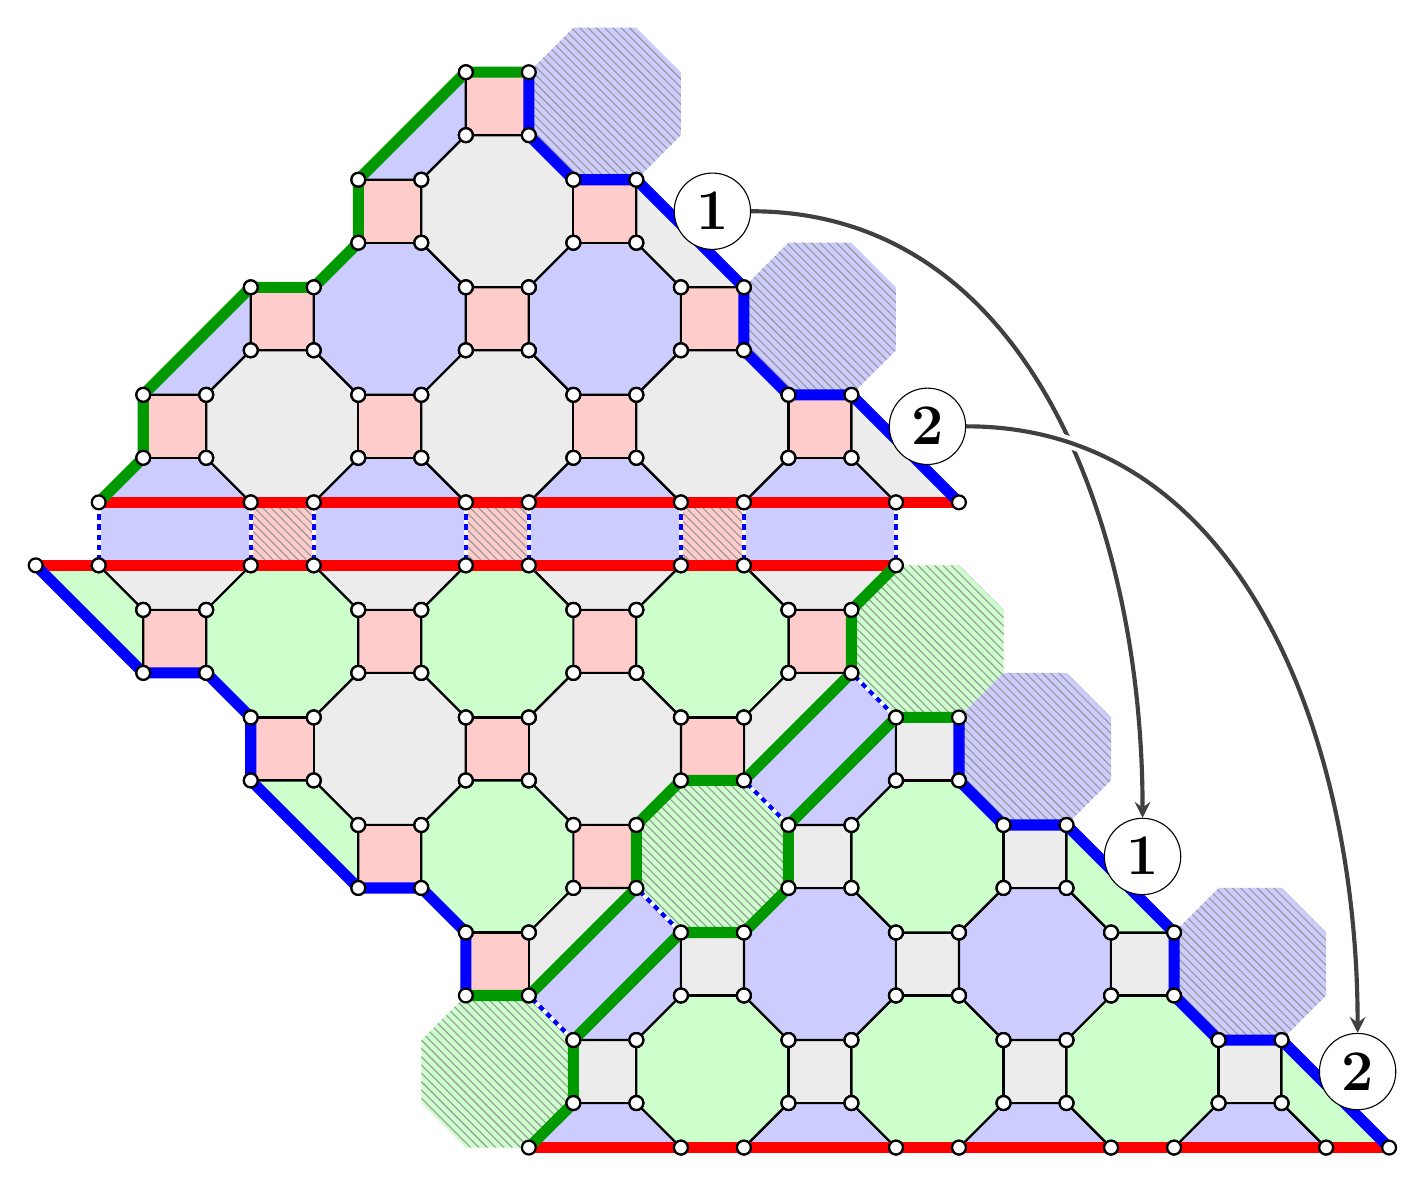
\begin{tikzpicture}
\def\L{1.3657}

\newcommand{\simplsq}[2]{
                \filldraw[colR] ({#1-0.4},{#2-0.4}) rectangle ({#1+0.4},{#2+0.4});
            }
            \newcommand{\simploct}[3]{
                \filldraw[#3]
                    ({#1-0.4},{#2-0.9657}) -- ({#1+0.4},{#2-0.9657}) -- ({#1+0.9657},{#2-0.4}) --
                    ({#1+0.9657},{#2+0.4}) -- ({#1+0.4},{#2+0.9657}) -- ({#1-0.4},{#2+0.9657}) --
                    ({#1-0.9657},{#2+0.4}) -- ({#1-0.9657},{#2-0.4}) -- cycle;
            }
            \newcommand{\simpltrapBtop}[2]{
                \filldraw[colB]
                    ({#1-0.9657},{#2+0.4}) -- ({#1-0.4},{#2+0.9657}) -- 
                    ({#1+0.4},{#2+0.9657}) -- ({#1+0.9657},{#2+0.4}) -- cycle;
            }
            \newcommand{\simpltrapBright}[2]{
                \filldraw[colB]
                    ({#1+0.9657},{#2+0.4}) -- ({#1+0.9657},{#2-0.4}) -- 
                    ({#1+0.4},{#2-0.9657}) -- ({#1-0.4},{#2-0.9657}) -- cycle;
            }
            \newcommand{\simpltrapGleft}[2]{
                \filldraw[colG]
                    ({#1-0.9657},{#2+0.4}) -- ({#1-0.9657},{#2-0.4}) -- 
                    ({#1-0.4},{#2-0.9657}) -- ({#1+0.4},{#2-0.9657}) -- cycle;
            }
            
            \newcommand{\fullsqqubits}[2]{
                \filldraw[fill=white, draw=black, thick] ({#1-0.4},{#2-0.4}) circle (2.5pt);
                \filldraw[fill=white, draw=black, thick] ({#1+0.4},{#2-0.4}) circle (2.5pt);
                \filldraw[fill=white, draw=black, thick] ({#1+0.4},{#2+0.4}) circle (2.5pt);
                \filldraw[fill=white, draw=black, thick] ({#1-0.4},{#2+0.4}) circle (2.5pt);
            }
            \newcommand{\fulloctqubits}[2]{
                \filldraw[fill=white, draw=black, thick] ({#1-0.4},{#2-0.9657}) circle (2.5pt);
                \filldraw[fill=white, draw=black, thick] ({#1+0.4},{#2-0.9657}) circle (2.5pt);
                \filldraw[fill=white, draw=black, thick] ({#1+0.9657},{#2-0.4}) circle (2.5pt);
                \filldraw[fill=white, draw=black, thick] ({#1+0.9657},{#2+0.4}) circle (2.5pt);
                \filldraw[fill=white, draw=black, thick] ({#1+0.4},{#2+0.9657}) circle (2.5pt);
                \filldraw[fill=white, draw=black, thick] ({#1-0.4},{#2+0.9657}) circle (2.5pt);
                \filldraw[fill=white, draw=black, thick] ({#1-0.9657},{#2+0.4}) circle (2.5pt);
                \filldraw[fill=white, draw=black, thick] ({#1-0.9657},{#2-0.4}) circle (2.5pt);
            }
            \newcommand{\trapBtopqubits}[2]{
                \filldraw[fill=white, draw=black, thick] ({#1-0.9657},{#2+0.4}) circle (2.5pt);
                \filldraw[fill=white, draw=black, thick] ({#1-0.4},{#2+0.9657}) circle (2.5pt);
                \filldraw[fill=white, draw=black, thick] ({#1+0.4},{#2+0.9657}) circle (2.5pt);
                \filldraw[fill=white, draw=black, thick] ({#1+0.9657},{#2+0.4}) circle (2.5pt);
            }
            \newcommand{\trapBrightqubits}[2]{
                \filldraw[fill=white, draw=black, thick] ({#1+0.9657},{#2+0.4}) circle (2.5pt);
                \filldraw[fill=white, draw=black, thick] ({#1+0.9657},{#2-0.4}) circle (2.5pt);
                \filldraw[fill=white, draw=black, thick] ({#1+0.4},{#2-0.9657}) circle (2.5pt);
                \filldraw[fill=white, draw=black, thick] ({#1-0.4},{#2-0.9657}) circle (2.5pt);
            }
            \newcommand{\trapGleftqubits}[2]{
                \filldraw[fill=white, draw=black, thick] ({#1-0.9657},{#2+0.4}) circle (2.5pt);
                \filldraw[fill=white, draw=black, thick] ({#1-0.9657},{#2-0.4}) circle (2.5pt);
                \filldraw[fill=white, draw=black, thick] ({#1-0.4},{#2-0.9657}) circle (2.5pt);
                \filldraw[fill=white, draw=black, thick] ({#1+0.4},{#2-0.9657}) circle (2.5pt);
            }

            

\newcommand{\drawLattice}[1]{
    \begin{scope}[#1]
        \simpltrapBtop{-3*\L}{0}
            \simpltrapBtop{-\L}{0}
            \simpltrapBtop{\L}{0}
            \simpltrapBtop{3*\L}{0}

            \simplsq{-3*\L}{\L}
            \simploct{-2*\L}{\L}{colG}
            \simplsq{-\L}{\L}
            \simploct{0}{\L}{colG}
            \simplsq{\L}{\L}
            \simploct{2*\L}{\L}{colG}
            \simplsq{3*\L}{\L}
            \simpltrapGleft{4*\L}{\L}

            \simpltrapBright{-3*\L}{2*\L}
            \simplsq{-2*\L}{2*\L}
            \simploct{-\L}{2*\L}{colB}
            \simplsq{0}{2*\L}
            \simploct{\L}{2*\L}{colB}
            \simplsq{2*\L}{2*\L}

            \simplsq{-\L}{3*\L}
            \simploct{0}{3*\L}{colG}
            \simplsq{\L}{3*\L}
            \simpltrapGleft{2*\L}{3*\L}

            \simpltrapBright{-\L}{4*\L}
            \simplsq{0}{4*\L}

            
    \end{scope}
}

\newcommand{\drawQubits}[1]{
    \begin{scope}[#1]
        \trapBtopqubits{-3*\L}{0}
            \trapBtopqubits{-\L}{0}
            \trapBtopqubits{\L}{0}
            \trapBtopqubits{3*\L}{0}

            \fullsqqubits{-3*\L}{\L}
            \fulloctqubits{-2*\L}{\L}
            \fullsqqubits{-\L}{\L}
            \fulloctqubits{0}{\L}
            \fullsqqubits{\L}{\L}
            \fulloctqubits{2*\L}{\L}
            \fullsqqubits{3*\L}{\L}
            \trapGleftqubits{4*\L}{\L}

            \trapBrightqubits{-3*\L}{2*\L}
            \fullsqqubits{-2*\L}{2*\L}
            \fulloctqubits{-\L}{2*\L}
            \fullsqqubits{0}{2*\L}
            \fulloctqubits{\L}{2*\L}
            \fullsqqubits{2*\L}{2*\L}

            \fullsqqubits{-\L}{3*\L}
            \fulloctqubits{0}{3*\L}
            \fullsqqubits{\L}{3*\L}
            \trapGleftqubits{2*\L}{3*\L}

            \trapBrightqubits{-\L}{4*\L}
            \fullsqqubits{0}{4*\L}

            
    \end{scope}
}

\colorlet{cR}{red!20}
\colorlet{cG}{green!20}
\colorlet{cB}{blue!20}

\colorlet{hideC}{gray!15}

\def\hideOp{1.0}
\def\showOp{1.0}

% T3: RB (Hide G) -> Points UP
\tikzset{
    colR/.style={fill=cR, draw=black, thick, solid, fill opacity=\showOp},
    colG/.style={fill=hideC, draw=black, thick, solid, fill opacity=\hideOp},
    colB/.style={fill=cB, draw=black, thick, solid, fill opacity=\showOp}
}
\drawLattice{shift={(0,0)}}

% T1: RG (Hide B) -> Points DOWN
\tikzset{
    colR/.style={fill=cR, draw=black, thick, solid, fill opacity=\showOp},
    colG/.style={fill=cG, draw=black, thick, solid, fill opacity=\showOp},
    colB/.style={fill=hideC, draw=black, thick, solid, fill opacity=\hideOp}
}
\drawLattice{shift={(0,0)}, rotate=180}

% T2: GB (Hide R) -> Points UP
\tikzset{
    colR/.style={fill=hideC, draw=black, thick, solid, fill opacity=\hideOp},
    colG/.style={fill=cG, draw=black, thick, solid, fill opacity=\showOp},
    colB/.style={fill=cB, draw=black, thick, solid, fill opacity=\showOp}
}
\drawLattice{shift={(4*\L, -6*\L)}}

% SEWING RED BOUNDARY (RB and RG)
\foreach \x in {-2, 0, 2} {
    \filldraw[fill=cR, draw=none] (\x*\L-0.4, -0.4) rectangle (\x*\L+0.4, 0.4);
    \filldraw[pattern=north west lines, pattern color=gray!80, draw=none] (\x*\L-0.4, -0.4) rectangle (\x*\L+0.4, 0.4);
}
\foreach \x in {-3, -1, 1, 3} {
    \filldraw[fill=cB, draw=black, thick] (\x*\L-0.9657, -0.4) rectangle (\x*\L+0.9657, 0.4);
    \draw[blue, line width=1.5pt] (\x*\L-0.9657, -0.4) -- (\x*\L-0.9657, 0.4);
    \draw[white, dash pattern=on 1.7pt off 2pt, line width=1.5pt] (\x*\L-0.9657, -0.4) -- (\x*\L-0.9657, 0.4);
    \draw[blue, line width=1.5pt] (\x*\L+0.9657, -0.4) -- (\x*\L+0.9657, 0.4);
    \draw[white, dash pattern=on 1.7pt off 2pt, line width=1.5pt] (\x*\L+0.9657, -0.4) -- (\x*\L+0.9657, 0.4);
}

% SEWING GREEN BOUNDARY (RG and GB)
% 1. Virtual Green octagons
\foreach \x/\y in {0/-5, 2/-3, 4/-1} {
    \filldraw[fill=cG, draw=none]
        ({\x*\L-0.4},{\y*\L+0.9657}) -- ({\x*\L+0.4},{\y*\L+0.9657}) -- 
        ({\x*\L+0.9657},{\y*\L+0.4}) -- ({\x*\L+0.9657},{\y*\L-0.4}) -- 
        ({\x*\L+0.4},{\y*\L-0.9657}) -- ({\x*\L-0.4},{\y*\L-0.9657}) -- 
        ({\x*\L-0.9657},{\y*\L-0.4}) -- ({\x*\L-0.9657},{\y*\L+0.4}) -- cycle;
    
    \filldraw[pattern=north west lines, pattern color=gray!80, draw=none]
        ({\x*\L-0.4},{\y*\L+0.9657}) -- ({\x*\L+0.4},{\y*\L+0.9657}) -- 
        ({\x*\L+0.9657},{\y*\L+0.4}) -- ({\x*\L+0.9657},{\y*\L-0.4}) -- 
        ({\x*\L+0.4},{\y*\L-0.9657}) -- ({\x*\L-0.4},{\y*\L-0.9657}) -- 
        ({\x*\L-0.9657},{\y*\L-0.4}) -- ({\x*\L-0.9657},{\y*\L+0.4}) -- cycle;
}

% 2. Sew Blue trapezoids
\foreach \x/\y in {1/-4, 3/-2} {
    \filldraw[fill=cB, draw=black, thick] (\x*\L+0.4, \y*\L+0.9657) -- (\x*\L-0.9657, \y*\L-0.4) -- (\x*\L-0.4, \y*\L-0.9657) -- (\x*\L+0.9657, \y*\L+0.4) -- cycle;
    
    \draw[blue, line width=1.5pt] (\x*\L+0.4, \y*\L+0.9657) -- (\x*\L+0.9657, \y*\L+0.4);
    \draw[white, dash pattern=on 1.7pt off 2pt, line width=1.5pt] (\x*\L+0.4, \y*\L+0.9657) -- (\x*\L+0.9657, \y*\L+0.4);
    
    \draw[blue, line width=1.5pt] (\x*\L-0.9657, \y*\L-0.4) -- (\x*\L-0.4, \y*\L-0.9657);
    \draw[white, dash pattern=on 1.7pt off 2pt, line width=1.5pt] (\x*\L-0.9657, \y*\L-0.4) -- (\x*\L-0.4, \y*\L-0.9657);
}

% --- MARKING THE THIRD CONNECTION (BLUE BOUNDARY) ---

% Virtual Blue octagons on RB
\foreach \x/\y in {3/2, 1/4} {
    \filldraw[fill=cB, draw=none]
        ({\x*\L-0.4},{\y*\L+0.9657}) -- ({\x*\L+0.4},{\y*\L+0.9657}) -- 
        ({\x*\L+0.9657},{\y*\L+0.4}) -- ({\x*\L+0.9657},{\y*\L-0.4}) -- 
        ({\x*\L+0.4},{\y*\L-0.9657}) -- ({\x*\L-0.4},{\y*\L-0.9657}) -- 
        ({\x*\L-0.9657},{\y*\L-0.4}) -- ({\x*\L-0.9657},{\y*\L+0.4}) -- cycle;
    \filldraw[pattern=north west lines, pattern color=gray!80, draw=none]
        ({\x*\L-0.4},{\y*\L+0.9657}) -- ({\x*\L+0.4},{\y*\L+0.9657}) -- 
        ({\x*\L+0.9657},{\y*\L+0.4}) -- ({\x*\L+0.9657},{\y*\L-0.4}) -- 
        ({\x*\L+0.4},{\y*\L-0.9657}) -- ({\x*\L-0.4},{\y*\L-0.9657}) -- 
        ({\x*\L-0.9657},{\y*\L-0.4}) -- ({\x*\L-0.9657},{\y*\L+0.4}) -- cycle;
}

% Virtual Blue octagons on GB
\foreach \x/\y in {7/-4, 5/-2} {
    \filldraw[fill=cB, draw=none]
        ({\x*\L-0.4},{\y*\L+0.9657}) -- ({\x*\L+0.4},{\y*\L+0.9657}) -- 
        ({\x*\L+0.9657},{\y*\L+0.4}) -- ({\x*\L+0.9657},{\y*\L-0.4}) -- 
        ({\x*\L+0.4},{\y*\L-0.9657}) -- ({\x*\L-0.4},{\y*\L-0.9657}) -- 
        ({\x*\L-0.9657},{\y*\L-0.4}) -- ({\x*\L-0.9657},{\y*\L+0.4}) -- cycle;
    \filldraw[pattern=north west lines, pattern color=gray!80, draw=none]
        ({\x*\L-0.4},{\y*\L+0.9657}) -- ({\x*\L+0.4},{\y*\L+0.9657}) -- 
        ({\x*\L+0.9657},{\y*\L+0.4}) -- ({\x*\L+0.9657},{\y*\L-0.4}) -- 
        ({\x*\L+0.4},{\y*\L-0.9657}) -- ({\x*\L-0.4},{\y*\L-0.9657}) -- 
        ({\x*\L-0.9657},{\y*\L-0.4}) -- ({\x*\L-0.9657},{\y*\L+0.4}) -- cycle;
}

% DRAW ALL BOUNDARIES ON TOP
\begin{scope}[shift={(0,0)}]

                \draw[red, line width=4pt, line cap=round] 
                    ({-3*\L-0.9657}, 0.4) -- ({4*\L+0.4}, 0.4);

                \draw[green!60!black, line width=4pt, rounded corners=1pt, line cap=round]
                    ({-3*\L-0.9657}, 0.4) 
                    -- ({-3*\L-0.4}, 0.9657)
                    -- ({-3*\L-0.4}, {\L+0.4})
                    -- ({-2*\L-0.4}, {2*\L+0.4})
                    -- ({-2*\L+0.4}, {2*\L+0.4})
                    -- ({-\L-0.4}, {3*\L-0.4})
                    -- ({-\L-0.4}, {3*\L+0.4})
                    -- ({-0.4}, {4*\L+0.4})
                    -- ({0.4}, {4*\L+0.4});

                \draw[blue, line width=4pt, rounded corners=1pt, line cap=round]
                    ({4*\L+0.4}, 0.4)
                    -- ({3*\L+0.4}, {\L+0.4})
                    -- ({3*\L-0.4}, {\L+0.4})
                    -- ({2*\L+0.4}, {2*\L-0.4})
                    -- ({2*\L+0.4}, {2*\L+0.4})
                    -- ({\L+0.4}, {3*\L+0.4})
                    -- ({\L-0.4}, {3*\L+0.4})
                    -- ({0.4}, {4*\L-0.4})
                    -- ({0.4}, {4*\L+0.4});
            
\end{scope}
\begin{scope}[shift={(0,0)}, rotate=180]

                \draw[red, line width=4pt, line cap=round] 
                    ({-3*\L-0.9657}, 0.4) -- ({4*\L+0.4}, 0.4);

                \draw[green!60!black, line width=4pt, rounded corners=1pt, line cap=round]
                    ({-3*\L-0.9657}, 0.4) 
                    -- ({-3*\L-0.4}, 0.9657)
                    -- ({-3*\L-0.4}, {\L+0.4})
                    -- ({-2*\L-0.4}, {2*\L+0.4})
                    -- ({-2*\L+0.4}, {2*\L+0.4})
                    -- ({-\L-0.4}, {3*\L-0.4})
                    -- ({-\L-0.4}, {3*\L+0.4})
                    -- ({-0.4}, {4*\L+0.4})
                    -- ({0.4}, {4*\L+0.4});

                \draw[blue, line width=4pt, rounded corners=1pt, line cap=round]
                    ({4*\L+0.4}, 0.4)
                    -- ({3*\L+0.4}, {\L+0.4})
                    -- ({3*\L-0.4}, {\L+0.4})
                    -- ({2*\L+0.4}, {2*\L-0.4})
                    -- ({2*\L+0.4}, {2*\L+0.4})
                    -- ({\L+0.4}, {3*\L+0.4})
                    -- ({\L-0.4}, {3*\L+0.4})
                    -- ({0.4}, {4*\L-0.4})
                    -- ({0.4}, {4*\L+0.4});
            
\end{scope}
\begin{scope}[shift={(4*\L, -6*\L)}]

                \draw[red, line width=4pt, line cap=round] 
                    ({-3*\L-0.9657}, 0.4) -- ({4*\L+0.4}, 0.4);

                \draw[green!60!black, line width=4pt, rounded corners=1pt, line cap=round]
                    ({-3*\L-0.9657}, 0.4) 
                    -- ({-3*\L-0.4}, 0.9657)
                    -- ({-3*\L-0.4}, {\L+0.4})
                    -- ({-2*\L-0.4}, {2*\L+0.4})
                    -- ({-2*\L+0.4}, {2*\L+0.4})
                    -- ({-\L-0.4}, {3*\L-0.4})
                    -- ({-\L-0.4}, {3*\L+0.4})
                    -- ({-0.4}, {4*\L+0.4})
                    -- ({0.4}, {4*\L+0.4});

                \draw[blue, line width=4pt, rounded corners=1pt, line cap=round]
                    ({4*\L+0.4}, 0.4)
                    -- ({3*\L+0.4}, {\L+0.4})
                    -- ({3*\L-0.4}, {\L+0.4})
                    -- ({2*\L+0.4}, {2*\L-0.4})
                    -- ({2*\L+0.4}, {2*\L+0.4})
                    -- ({\L+0.4}, {3*\L+0.4})
                    -- ({\L-0.4}, {3*\L+0.4})
                    -- ({0.4}, {4*\L-0.4})
                    -- ({0.4}, {4*\L+0.4});
            
\end{scope}

% DRAW QUBITS ON TOP OF BOUNDARIES
\drawQubits{shift={(0,0)}}
\drawQubits{shift={(0,0)}, rotate=180}
\drawQubits{shift={(4*\L, -6*\L)}}

% Numbering Green boundary shapes to indicate the Möbius twist
\tikzset{
    twistNode/.style={circle, fill=white, draw=black, inner sep=3.5pt, font=\bfseries\huge}
}

% On RB (Right edge) - 1 is top, 2 is bottom
\node[twistNode] (RB1) at (2*\L, 3*\L) {1};
\node[twistNode] (RB2) at (4*\L, \L) {2};

% On GB (Right edge) - 1 is top, 2 is bottom
\node[twistNode] (GB1) at (6*\L, -3*\L) {1};
\node[twistNode] (GB2) at (8*\L, -5*\L) {2};

% Twist connection arrows
\draw[->, >=stealth, darkgray, thick, line width=1.5pt] (RB1) to[out=0, in=90] (GB1);
\draw[white, line width=4.5pt] (RB2) to[out=0, in=90] (GB2); % White outline for 3D crossing effect
\draw[->, >=stealth, darkgray, thick, line width=1.5pt] (RB2) to[out=0, in=90] (GB2);

\end{tikzpicture}
}
        \caption{Unified M\"obius topology}
        \label{fig:mobius_c}
    \end{subfigure}
    \caption[M\"obius strip construction from 2D color code restrictions]{
        M\"obius strip construction from 2D color code restrictions. 
        (a) The original planar color code lattice. Outer boundaries are highlighted in their respective colors.
        (b) Independent restriction decoders generated by eliminating one color at a time (RB, RG, and GB patches).
        (c) Unified lattice showing the topological connections. The RB and RG patches are sewn along their red boundary, while RG and GB are sewn along their green boundary. Virtual boundary stabilizers (patterned) fill the resulting topological gaps. The twist required to connect the remaining blue boundaries of RB and GB forms a M\"obius strip, matching the numbered detectors.
    }
    \label{fig:mobius_unified_lattice}
\end{figure}

\end{document}
